\addcontentsline{toc}{chapter}{\numberline{}{Portada}}

\pagenumbering{roman} \setcounter{page}{1}

%--
\thispagestyle{empty}
%\includepdf[pages=-,link=true,landscape,linkname=PortadaPastas]{capitulo10/pdf_portada_prueba2}

%\cleardoublepage NO METER
%\thispagestyle{empty} NO METER
%\clearpage{\pagestyle{empty}\cleardoublepage} NO METER
%--
\newpage

\thispagestyle{empty}

\begin{center}
\textbf{\huge 
\includegraphics[scale=0.8]{logo_ugr.png}}
\par\end{center}{\huge \par}

\begin{center}
\vspace*{1cm} 
\par\end{center}

\begin{center}
\textbf{\large ESTUDIOS DE INGENIERÍA }\\
\textbf{\large DE TELECOMUNICACIÓN}
\par\end{center}{\large \par}

\begin{center}
\textbf{\large PROYECTO FIN DE CARRERA}
\par\end{center}{\large \par}

\begin{center}

\par\end{center}

\begin{center}
\textbf{\emph{\LARGE {}``Control de temperatura en un horno con un microcontrolador''}}
\par\end{center}{\LARGE \par}

\begin{center}
\vspace*{3cm} 
\par\end{center}

\begin{center}
{\large CURSO: 2014/2015}
\par\end{center}{\large \par}

\begin{center}
{\large Germán del Castillo Cuesta}
\par\end{center}{\large \par}

\newpage
\thispagestyle{empty}

~

\newpage
\thispagestyle{empty}

\begin{center}

\includegraphics[scale=0.8]{logo_ugr.png}
\par\end{center}

\begin{center}
ESTUDIOS DE INGENIERÍA DE TELECOMUNICACIÓN
\par\end{center}

\begin{center}
\vspace*{0.1cm}
\par\end{center}

\begin{center}
\textbf{\emph{\Large {}``Control de temperatura en un horno con un microcontrolador''}}
\par\end{center}{\Large \par}

\begin{center}
\vspace*{0.3cm}
\par\end{center}

\begin{center}
REALIZADO POR:
\par\end{center}

\begin{center}
\textbf{Germán del Castillo Cuesta}
\par\end{center}

\begin{center}
DIRIGIDO POR:
\par\end{center}

\begin{center}
\textbf{Andrés María Roldán Aranda}
\par\end{center}

\begin{center}
DEPARTAMENTO:
\par\end{center}

\begin{center}
\textbf{Electrónica y Tecnología de los Computadores}
\par\end{center}

\begin{center}
\vfill 
\par\end{center}


%\lyxrightaddress{Granada, Julio de 2012}

\vspace*{1.5cm}

\newpage
\thispagestyle{empty}

~

%%Begin ----  Para que funcione bien el TOC en PDF
%\cleardoublepage
%\phantomsection
%\thispagestyle{empty}
%%\chapter*{Hoja de Firmas}
%
%\addcontentsline{toc}{chapter}{Hoja de Firmas}
%
%\begin{center}
%
\includegraphics[scale=0.8]{logo_ugr.png}
%\par\end{center}
%
%\begin{center}
%ESTUDIOS DE INGENIERÍA DE TELECOMUNICACIÓN
%\par\end{center}
%
%\begin{center}
%\vspace*{0.1cm}
%\par\end{center}
%
%\begin{center}
%\textbf{\emph{\Large {}``Sistema de caracterización de dispositivos magnetorresistivos''}}
%\par\end{center}{\Large \par}
%
%\begin{center}
%\vspace*{0.2cm}
%\par\end{center}
%
%\begin{center}
%REALIZADO POR:
%\par\end{center}
%
%\begin{center}
%\textbf{Ignacio Rodríguez López}
%\par\end{center}
%
%\begin{center}
%TRIBUNAL:
%\par\end{center}
%
%\textbf{D/Dña} \hrulefill{}~\hspace{1.5cm}\\
%
%
%\textbf{D}/\textbf{Dña }\hrulefill{}~\hspace{1.5cm}\\
%
%
%\textbf{D/Dña }\hrulefill{}~\hspace{1.5cm}\\
%
%
%\begin{flushright}
%Presentado en Granada, a ~~~~~~ de Abril de 2013.\\
%Evaluado en Granada, a ~~~~~~ de Abril de 2013.
%\par\end{flushright}
%
%\noindent \begin{center}
%El Presidente\hspace{3cm}El Vocal\hspace{3cm}El Secretario
%\par\end{center}
%
%\newpage
%\thispagestyle{empty}

\begin{itemize}
	\item [] 
\end{itemize}


\newpage
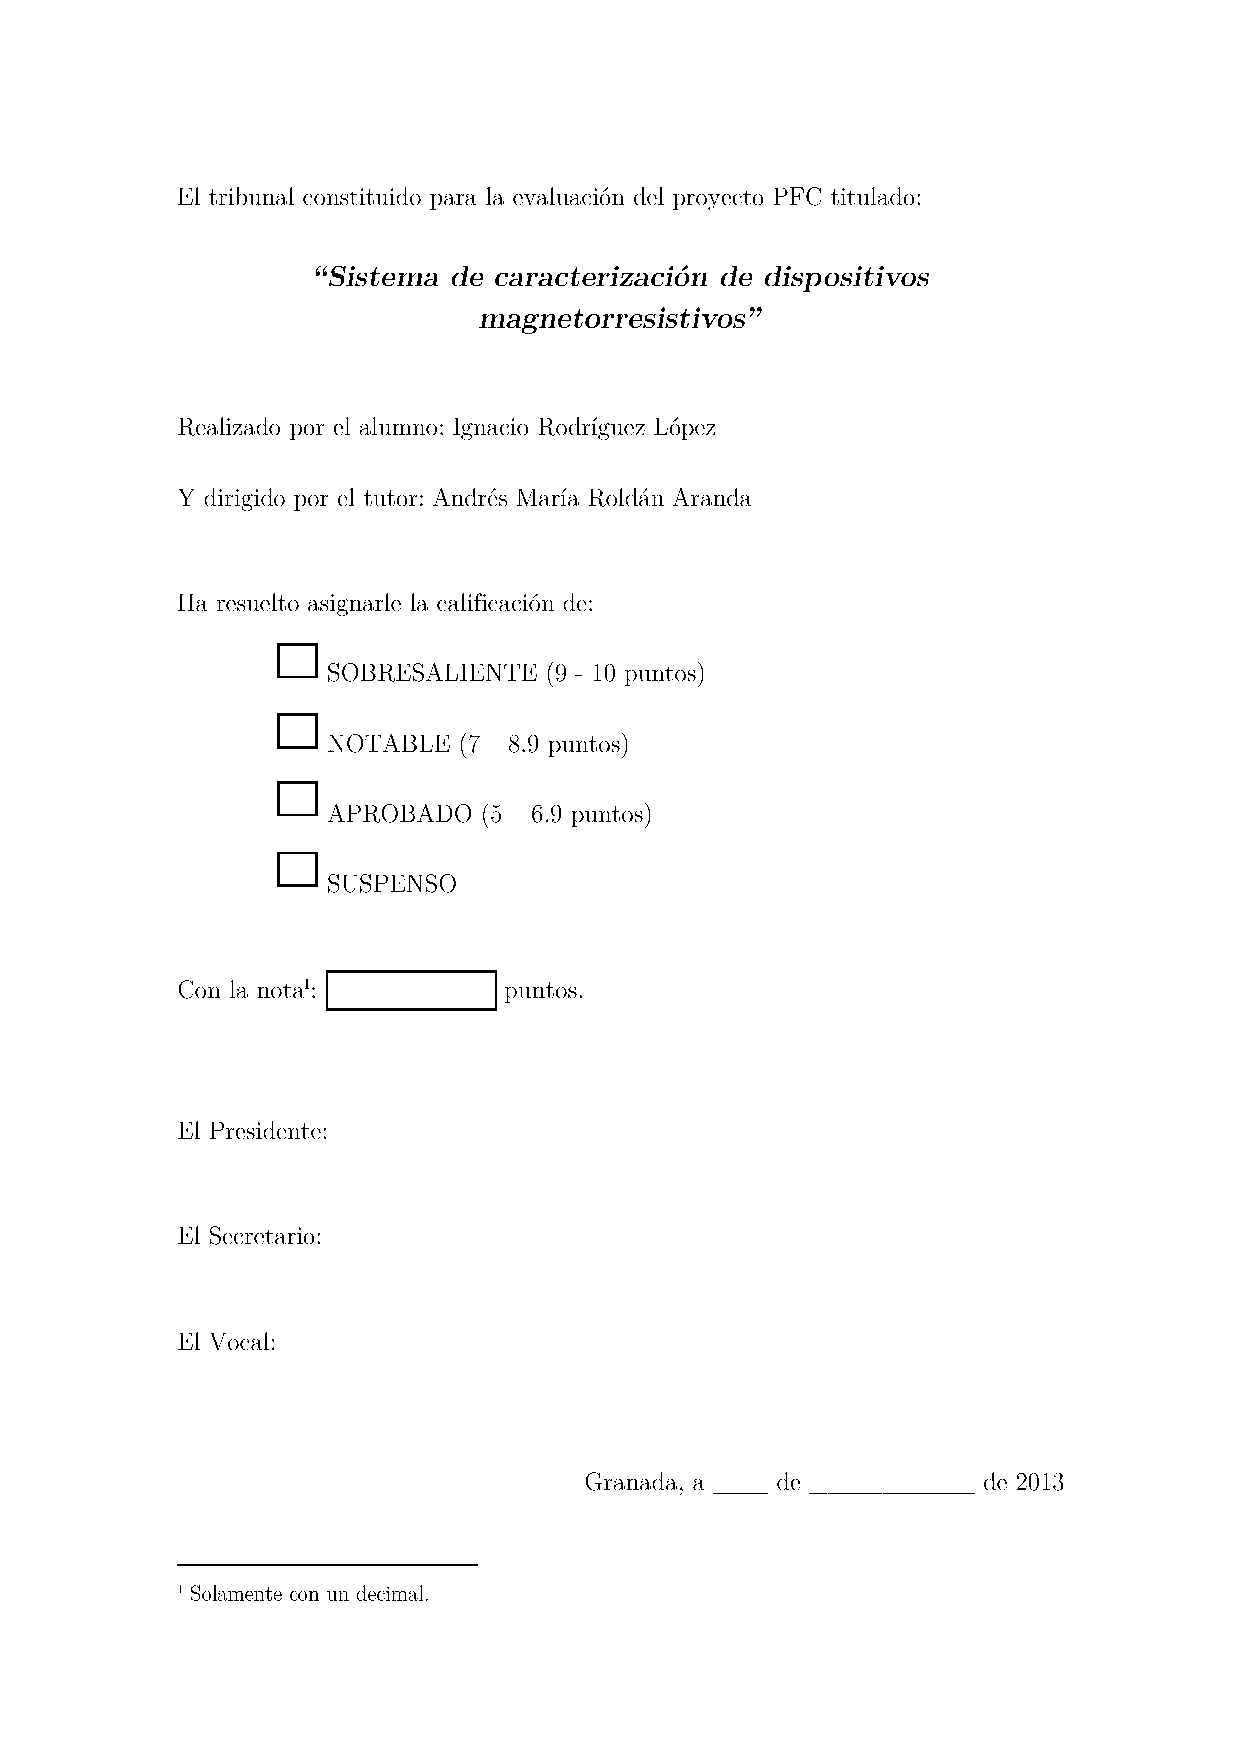
\includepdf[pages=-,link=true,linkname=hojaEvaluacionesUGR]{anexoIV_actaPFC}

\newpage
\thispagestyle{empty}

%Begin ----  Para que funcione bien el TOC en PDF
\cleardoublepage
\thispagestyle{empty}
\phantomsection
\addcontentsline{toc}{chapter}{Autorización Lectura}

\noindent D. Andrés María Roldán Aranda, Profesor del departamento
de Electrónica y Tecnología de los Computadores de la Universidad
de Granada, como director del Proyecto Fin de Carrera de D. Germán del Castillo Cuesta,

\vspace*{1cm}

Informa:

\begin{doublespace}
que el presente trabajo, titulado:
\end{doublespace}

\begin{doublespace}
\begin{center}
\textbf{\emph{\large {}``Control de temperatura en un horno con un microcontrolador''}}
\par\end{center}{\large \par}
\end{doublespace}

\noindent ha sido realizado y redactado por el mencionado alumno bajo
nuestra dirección, y con esta fecha autorizo a su presentación. 

\vspace*{1cm}

\begin{center}
%Granada, a 06 de Julio de 2012 
Granada, a ~~~~~~ de Junio de 2015
\par\end{center}

\bigskip%%%%%%%o
\bigskip%%%%%%%o
\begin{doublespace}
\hspace{4cm}Fdo.
\end{doublespace}

\newpage
\thispagestyle{empty}
\noindent

\newpage
\thispagestyle{empty}

~

%Begin ----  Para que funcione bien el TOC en PDF
\cleardoublepage
\phantomsection
\thispagestyle{empty}

\addcontentsline{toc}{chapter}{Autorización Depósito Biblioteca}

\noindent Los abajo firmantes autorizan a que la presente copia de
Proyecto Fin de Carrera se ubique en la Biblioteca del Centro y/o
departamento para ser libremente consultada por las personas que lo
deseen.

\vspace*{1cm}

\begin{center}
%Granada, a 06 de Julio de 2012
Granada, a ~~~~~~ de Junio de 2015
\par\end{center}

\bigskip%%%%%%%o
\bigskip%%%%%%%o
\begin{doublespace}
\hspace{4cm}Fdo.
\end{doublespace}

\newpage
\thispagestyle{empty}

~

%Begin ----  Para que funcione bien el TOC en PDF
\cleardoublepage
\phantomsection
\thispagestyle{empty}
\addcontentsline{toc}{chapter}{Resumen}

\begin{center}
\textbf{\Large Control de temperatura en un horno con un microcontrolador}
\par\end{center}{\Large \par}

\begin{center}
\textbf{\large Germán del Castillo Cuesta}
\par\end{center}{\large \par}

\vspace{0.75cm}






\begin{doublespace}
\noindent \textbf{PALABRAS CLAVE:}
\end{doublespace}



\begin{singlespace}
\noindent Arduino, PCB, PT100, PID, Matlab, Altium, Rotary Encoder, horno,SMD.

\end{singlespace}

\begin{doublespace}
\noindent \textbf{RESUMEN:}
\end{doublespace}

\begin{singlespace}

\noindent Este proyecto tendrá como objetivo la realización de un sistema de caracterización de dispositivos magnetorresistivos. El trabajo se concentrará en el diseño de un escenario capaz de posicionarse sobre dichos dispositivos e inducir en ellos un campo magnético homogéneo para analizar su comportamiento resistivo. El sistema incorporará un software específico para configurar el conexionado del sistema y lanzar el procedimiento de medida, controlando la instrumentación involucrada mediante buses GPIB y RS-232.
%Desarrollo de un sistema de control de puertas abatibles. El sistema estar? orientado hacia la unificaci?n en un solo producto de los distintos escenarios que existen en la realidad. Se dise?ar? el sistema completo, incluyendo desarrollos a nivel hardware y firmware. La recepci?n de las se?ales se har? desde un telecommando a la frecuencia reservada para ello.
\end{singlespace}

\vspace{1.25cm}


\begin{doublespace}
\noindent \textbf{KEYWORDS:}
\end{doublespace}

\begin{singlespace}
%\noindent Printed Circuit Board (PCB), control box, flap, RF communication, automation, microcontroller.
\noindent Magnetoresistance, sensors, magnetic field, Helmhotz's coils, current strap, characterisation, probe station, head probes, gaussmeter, Hall probes, Matlab, GPIB, RS-232, automation, simulation, remote control, electronic instrumentation, parameter analyzer, PCB.
\end{singlespace}

\begin{doublespace}
\noindent \textbf{ABSTRACT:}
\end{doublespace}

\begin{singlespace}
\noindent This project will develop a magnetoresistance devices characterisation system. This work will be focused on the design of an stage capable of positioning over these devices while inducing an homogeneous magnetic field on them in order to analyse their resistive behavior. The system will also integrate a specific software to assist the setup procedure as well as for triggering the measurement, remotely controlling all the involved intrumentation through GPIB and RS-232 buses. 
%\noindent Development of a folding door control. The system will be geared towards the unification into a single product of the different scenarios that exist in reality. It will design the entire system, including developments at the hardware and firmware. Receiving signals from a telecomm will the frequency reserved for it.
\end{singlespace}


\newpage
\thispagestyle{empty}

~

%Begin ----  Para que funcione bien el TOC en PDF
\cleardoublepage
\phantomsection
\thispagestyle{empty}
\addcontentsline{toc}{chapter}{Dedicatoria}

\vspace{6cm}

\begin{quotation}
\noindent \begin{center}
\textbf{\emph{\Large Dedicado a}}\textbf{\emph{\large }}\\
\textbf{\emph{\large }}\\
\textbf{\emph{\large }}\\
\textbf{\emph{\large Mis padres, Germán y Antonia. Sin ellos nada de esto hubiera sido posible.}}
%\textbf{\emph{\large .....Esto lo último.....}}
%Todos aquellos que no tuvieron la oportunidad.
\par\end{center}{\large \par}
\end{quotation}
\newpage
\thispagestyle{empty}

~\newpage
\thispagestyle{empty}


